%Chapter "Introduction"
%
\chapter{Introduction}

In an introductory graduate course in the Finite Element Method (FEM), the purpose is to develop a basic understanding of the discrete or numerical strategy of Finite Element-(FE) Algorithms when a closed form solution to a Boundary Value Problem (BVP) is not possible due to complexities existing probably: in the boundary conditions, material behavior or in the kinematic description used in the model. In such a course, in order to master and identify the main mathematical and algorithmic aspects of the method at the beginners level, the studied problem is kept lineal. In this sense 4 key aspects make the core of the introductory course (at least for the case of the linearized theory of elasticity boundary value problem):

\begin{itemize}

\item Formulation and identification of the strong form of the Boundary Value Problem (BVP) where the continuum mechanics governing equations are revisited and particularized to the case of linear elastic material behavior. The BVP is completed by identifying the correct prescription of boundary conditions for a well posed mathematical problem.

\item Formulation and identification of the weak form of the BVP where the governing equations and natural boundary conditions representing equilibrium at the material point level are replaced by an equivalent but weaker form of equilibrium now valid at the global level.  In the case of a Continuum Mechanics problem this so-called weak form can be shown to be equivalent to the principle of virtual power and lends itself for the partition of the problem into sub-domains or finite size elements.

\item Introduction of the idea of discretization dividing the problem into subdomains and using interpolation theory within each subdomain-In the context of the FE method this is the subject of shape functions. Once the computational specimen has been divided into subdomains (or a mesh of finite elements) the selected primary variable is approximated within each element via interpolation of the known response at selected predefined points or nodes.

\item Computational aspects grouped also into 5 points:
	\begin{itemize}
	\item Formulation of elemental matrices in the physical space.
	\item Formulation of elemental matrices in the natural domain-Isoparametric transformation.
	\item Numerical integration: Gauss quadrature.
	\item Assembly of system matrices and imposition of boundary conditions.
	\item Solution of the discrete equilibrium statement and calculation of elemental results.
	\end{itemize}
\end{itemize}

These 4 key points are perfectly well documented in numerous nicely written textbooks and it could be argued that is not even worth to register for an introductory course since a moderately dedicated student can accomplish the task via self-study. Unfortunately, linearity is scarce--although useful to grasp the basic understanding of the problem--and the real world is full of non-linear behavior and understanding the needed algorithms can be easily justified. In this \textcolor{red}{Advanced Finite Element Methods course} the goal is then to understand the basic aspects of non-linear finite element analysis.  Like in the linear case there is also a vast amount of literature for the non-linear problem.  However, in the non-linear case the kinematic problem itself may take different routes leading to a wide variety of FEM formulations that will difficult a self-study strategy.  Considering the above this brief set of class notes is intended as a guide for self-study and more important represents a help towards the implementation of the algorithm for the consideration of Material and Geometric Non-linearities in Solids.

The basic reference is Professor Bathe's textbook \cite{book:bathe} but we will also follow closely ABAQUS Theory Manual \cite{abaqus_theory}. ABAQUS is a robust, multi-physics oriented commercially available finite element analysis tool. Its strength resides in the effective non-linear algorithms and on the capability of taking user subroutines written in good old Fortran or in C++.  The possibility of implementing user subroutines makes it a very powerful research tool.  In the particular case of a stress/displacement analysis problem with non-linearities these are considered through the kinematics contribution or through the material contribution.  In the first case the non-linear behavior must be considered at the element level while in the second it corresponds to the response of a material point which in the context of the FEM algorithm corresponds to an integration point. In ABAQUS those two sources of non-linearity can be independently controlled by the user via user subroutines UEL and UMAT.  In both cases the non-linearity is primarily solved by the classical Newton-Raphson scheme and that will be the approached followed herein.  Although the notes are mainly written for an advanced course the specific problem of a linear solid usually studied in the introductory course can be derived like a particular case of the most general non-linear algorithm.

The current set of Class Notes is organized as follows.  First and since we will be dealing with history dependent non-linear problems the most powerful (at least when it works) solution algorithm, namely the Newton-Raphson iteration is studied.  The technique is first illustrated for the simple 1D-case and then generalized into the multi-degree of freedom system.  In both cases pseudo-codes will be presented preparing the way for the Finite Element Algorithm.  The presentation however is not exhaustive in mathematical terms and the reader is referred to excellent treatments like Burden \cite{book:burden2011} and Press et al. \cite{book:numerical_recipes} for the mathematical aspects of the Newton method.

In the next section the briefly introduced Newton-Raphson technique is contextualized to the case of a system of equations representing equilibrium between internal and external forces as typically found in a finite element model.  Moreover, the non-linearities come into play through a dependence of the internal forces into displacements.  At this stage the details of the formulation of the finite element equations via discretization into nodal variables is not presented but emphasis is laid down into the solution algorithm.  Interest is then given to the particular form taken by the Newton-Raphson algorithm into the commercial finite element code ABAQUS.  That code can be used as a powerful non-linear equation solver where the coefficient matrix and the excitation can be directly controlled by the user.  Moreover the solver can be used into a multi-physics context in terms of generalized forces and fluxes.  In the particular case of the stress analysis finite element method the user can control the elemental contribution to the coefficient matrix and the contribution of each material point to obtain that element contribution.  This is achieved through the so-called user subroutines UEL  for element and UMAT  for material.  Having introduced the Newton-Raphson method the notes concentrate next on general discretization aspects starting from the physical strong form of the equations in the deformed configuration and passing to an arbitrary weak form in the reference configuration.  The resulting algorithm is therefore a Total Lagrangian (TL) method.  Once the general equations are introduced a particular work conjugate stress-strain pair is chosen and the discrete equations, including kinematic interpolators, are described.

\section*{Notation}
In a non-linear algorithm the bookkeeping is involved since we have to simultaneously record 4 different fields as follows:
\begin{itemize}
	\item The physical fields in terms of tensorial descriptions.
	\item The time field since the problem is solved incrementally 	and time may appear as an artificial chronological variable 	or as a real quantity in a dynamic problem.
	\item The interpolation field.  Since all the involved variables will be interpolated we will need to keep track of the way this interpolation is being performed.
	\item The iterations field needed in the solution of the non-linear problem.
\end{itemize}
In order to keep this bookkeeping simple we use the following indicial notation with subscripts and superscripts

\begin{figure}[h]
\centering
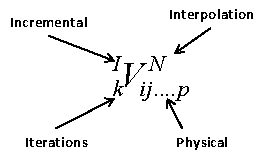
\includegraphics[width=4cm]{img/figure1_1.pdf}
\caption{General notation to study non-linear finite element problems}
\label{fig:notation}
\end{figure}

\textcolor{red}{Capital superscripts will be reserved for the incremental time description and for the interpolation scheme.  For instance an expression like   refers to the time instant   while   refers to . Similarly a variable   refers to interpolation over the node. Left and right subscripts will be used to make reference to the iteration being performed and the order of the tensorial variable.  For instance   refers to a second order tensor corresponding to the iteration.}